\documentclass[a4paper, oneside, 11pt]{article}
%% -> Für längere Arbeiten "report" benutzen.

%% --------------------------------------------------------------------- %%

\usepackage{ifthen}
\usepackage{svg}
\newboolean{english}
\setboolean{english}{false} %% -> Kommentar entfernen bei englischen Arbeiten

%% --------------------------------------------------------------------- %%

%% -> Einfügen der Definitionen
%% -> Deutsche Anpassung 
\usepackage[T1]{fontenc}
\usepackage[ngerman,english]{babel}
%\usepackage{babelbib}
\usepackage{ifthen}
%% --------------------------------------------------------------------- %%

%% -> Farben einfügen
\usepackage{color}
\usepackage{xcolor}

% -> Definierte Farben
\definecolor{MSBlue}{rgb}{.204,.353,.541} 
\definecolor{trueblue}{rgb}{0.0, 0.45, 0.81}
\definecolor{onyx}{rgb}{0.06, 0.06, 0.06}
\definecolor{mygruen}{rgb}{0.4660, 0.6740, 0.1880}
\definecolor{plotblue}{rgb}{0, 0.4470, 0.7410}
\definecolor{myrot}{rgb}{0.8500, 0.3250, 0.0980}
\definecolor{mygreen}{RGB}{28,172,0} %% Matlab Kommentar
\definecolor{mylilas}{RGB}{170,55,241} %% Matlab String

%% --------------------------------------------------------------------- %%

%% -> Grafiken 
\usepackage{graphicx}
\usepackage{epstopdf}
\usepackage{wallpaper}
\usepackage{float} 
\usepackage[section]%% Verbessert die Platzierung
%% --------------------------------------------------------------------- %%

\usepackage[tmargin=1in,bmargin=1in,lmargin=1.25in,rmargin=1.25in]{geometry}
\setlength{\parindent}{0em}
\setlength{\parskip}{1.5ex plus0.5ex minus0.5ex}
\usepackage{setspace}
\onehalfspacing

\usepackage{pst-all} %% erweiterte Zeichenbefehle

%% -> Schriftart
\usepackage{helvet}
\renewcommand{\familydefault}{phv}

%% -> Layout Überprüfung
\usepackage{layout}
\usepackage{xspace}

%% -> Für Tabellen
\usepackage{array}
\usepackage{booktabs}
\usepackage{dcolumn}
\usepackage{multirow}

%% -> Einrücken von und Abstand zwischen Absätzen
\setlength{\parindent}{0em}
\setlength{\parskip}{1.5ex plus0.5ex minus0.5ex}

%% -> Tabulator Funktion
\newcommand\tab[1][1cm]{\hspace*{#1}}

%% -> Weniger Warnungen wegen überfüllter Boxen
\tolerance = 9999
\sloppy

%% -> Erweiterte Einstellungen der Bildunterschriften bzw. Tabellenunterschriften
\usepackage{caption}
\usepackage{subcaption}
\captionsetup[figure]{labelfont=footnotesize, textfont=footnotesize}
\captionsetup[table]{labelfont=footnotesize, textfont=footnotesize}

%% -> Hyperref
\usepackage[pdftex,bookmarks=true,bookmarksnumbered=true,]{hyperref}

% \usepackage[hidelinks]{hyperref}
%\usepackage[colorlinks=true]{hyperref}
% \hypersetup{
% colorlinks=true,
% linkbordercolor={1 0 0},
% citebordercolor={0 1 0},
% filebordercolor={1 0 1},
% runbordercolor={1 0 1},
% urlbordercolor={0 0 1},
% }

%% -> Quellen
\usepackage[super, square, sort&compress]{natbib}

%%-> Weitere nützliche Pakete
\usepackage{todonotes}
\setlength {\marginparwidth }{2cm}
%% --------------------------------------------------------------------- %%

% -> Für Codes zum einfügen
\usepackage{listings}
%\lstset{numbers=left,numberstyle=\tiny,stepnumber=5,numbersep=5pt}

%% -> Für MATLAB Code
\lstset
{language=Matlab,%
    basicstyle=\scriptsize,
    breaklines=true,%
    captionpos=b,
    frame = single,
    morekeywords={matlab2tikz},
    keywordstyle=\color{blue},%
    morekeywords=[2]{1}, keywordstyle=[2]{\color{black}},
    identifierstyle=\color{black},%
    stringstyle=\color{mylilas},
    commentstyle=\color{mygreen},%
    showstringspaces=false,%
    %numbers=left,%
    %numberstyle={\footnotesize \color{black}},%
    %stepnumber=5, %
    %numbersep=9pt, % 
    emph=[1]{for,end,break},emphstyle=[1]\color{red}, %
    emph=[2]{all}, emphstyle=[2]\color{mylilas},    
}
%% --------------------------------------------------------------------- %%

% -> Kopf und Fußzeile gestallten
\usepackage{fancyhdr}
%\setlength{\headheight}{13.6pt}
\setlength{\footskip}{41pt}
\rhead{} 
\chead{} 
\lhead{}
\renewcommand{\headrulewidth}{0pt}
\lfoot{
\includegraphics[width=\textwidth*1/6]{Definition/DUH-positive.eps}}
\rfoot{\small\thepage}
\cfoot{}
\renewcommand{\footrulewidth}{0pt}
%% --------------------------------------------------------------------- %%

%% -> Matematische Packages
\usepackage{amsmath,amssymb,amsfonts,amstext}
\usepackage{mathtools}
\usepackage{mathrsfs}

%% -> SI-Einheiten
%\usepackage{units}
\usepackage{siunitx}
% \usepackage{physics}
\sisetup{locale = DE,separate-uncertainty}
\sisetup{list-final-separator={ und }}
\sisetup{per-mode=fraction}
\DeclareSIUnit\Pascal{\newton\per\square\metre}
%\sisetup{output-decimal-marker = {.}} %% Für Punkttrennung nur bei englischen Arbeiten erforderlich
%% --------------------------------------------------------------------- %%

%% -> Für die Überschriften
\usepackage{titlesec}
\titleformat{\section}{\LARGE\sffamily\bfseries}{\thesection}{1em}{}
\titleformat{\subsection}{\Large\bfseries\sffamily}{\thesubsection}{1em}{}
\titleformat{\subsubsection}{\large\sffamily\bfseries}{\thesubsubsection}{1em}{}
%% --------------------------------------------------------------------- %%

%% -> Bildnummerierung ist logisch mit Kapitelnummerierung
\numberwithin{figure}{section}
\numberwithin{table}{section}
\numberwithin{equation}{section}
%\numberwithin{equation}{subsection}
%% --------------------------------------------------------------------- %%

%% -> Schaltplan zeichnen und Grafiken und für PGF Plots
\usepackage[european, siunitx]{circuitikz}
\usepackage{tikz}
\usepackage{tikzscale}
\usepackage{pgfplots}
\pgfplotsset{compat=1.4}
\newlength\figH
\newlength\figW
\setlength{\figH}{6cm}
\setlength{\figW}{8cm}
%% --------------------------------------------------------------------- %%

%% -> Für das Formelverzeichnis
\DeclareCaptionType{myequations}[][Formelverzeichnis]
\captionsetup[myequations]{labelformat=empty}
%% --------------------------------------------------------------------- %%

%% -> Für das Symbolverzeichnis
\usepackage[toc, hyperfirst = false, acronym, nonumberlist]{glossaries}
\makeglossaries
%\input{Symbols_Acronym/symbols}
%\input{Symbols_Acronym/acronym}
%% --------------------------------------------------------------------- %%



%% -> Deckblatt ausfüllen 
\def\labtitle{Leadership Development}
\def\labcode{BB MECH-M-3-MSK-LED-SE}
\def\labname{}
\def\labnum{1}
\def\study{Master Mechatronik}
\def\branch{Smart Technologies}
\def\term{3.}
\def\lecturer{Claudia Mair}
\def\group{MA-MECH-23-BB}
\def\student{Sieß Lukas}

%% --------------------------------------------------------------------- %%

%% -> Beginn des Dokumentes

\begin{document}
\newcounter{romanPagenumber}

%% -> Sprache auswählen
\ifthenelse{\boolean{english}}{\selectlanguage{english}}{\selectlanguage{ngerman}}
% \selectlanguage{ngerman}
% \selectlanguage{english}

%% -> Fußzeile und Kopfzeile einfügen
\pagestyle{fancy}

\pagenumbering{Roman}
%% -> Deckblatt laden
%% Deckblatt %%

\thispagestyle{empty}
\sffamily
\ThisTileWallPaper{\paperwidth}{\paperheight}{Deckblatt/MCIHintergrundKPL.pdf}

\vspace*{1cm}
\def\thesis{\ifthenelse{\boolean{english}}{Abschlussbericht}{Aufgaben}}
\textcolor{MSBlue}{\rmfamily\bfseries\Huge\thesis}

\vspace*{0.5cm}
\textbf{\labtitle{} (\labcode)}

\textbf{\labname}

%\ifthenelse{\boolean{english}}{\textbf{Report} }{\textbf{Labor }}\textbf{\labnum}


\vspace*{14cm}

\textcolor{gray}{\study}

% \def\studybranch{\ifthenelse{\boolean{english}}{Study Branch}{Studienzweig}}
% \textcolor{gray}{\studybranch: \branch}

\def\termname{\ifthenelse{\boolean{english}}{semester}{Semester}}
\textcolor{gray}{\term{ }\termname}

\def\lecturername{\ifthenelse{\boolean{english}}{Responsible lecturer}{Lehrveranstaltungsleiter}}
\textcolor{gray}{\lecturername: \lecturer}

\def\groupname{\ifthenelse{\boolean{english}}{Group}{Jahrgang}}
\textcolor{gray}{\groupname: \group}

\def\authorname{\ifthenelse{\boolean{english}}{Author}{Verfasser}}
\textcolor{gray}{\authorname: \student}

\textcolor{gray}{\today}

\newpage

\setcounter{romanPagenumber}{\value{page}}

%% -> Inhaltsverzeichnis
\tableofcontents%\thispagestyle{empty}
\clearpage

\pagestyle{fancy}
\pagenumbering{arabic}

%% --------------------------------------------------------------------- %%
%% -> Anfang
\section{Myers-Briggs-Test}
Im Rahmen meines Myers-Briggs-Ergebnisses, das mich als ESTJ (Exekutive) beschreibt, zeigt sich, dass mein Führungsverhalten stark von Struktur, Effizienz und klaren Zielen geprägt ist. Diese Kernaspekte meines Persönlichkeitsprofils wirken sich durchweg positiv auf mein Handeln und meine Entscheidungsfindung aus, insbesondere in Führungsrollen. Der ESTJ-Typ legt großen Wert auf bewährte Methoden und etablierte Systeme, was mir hilft, Ordnung und Stabilität in meinen Teams zu schaffen.
Im Kontext des LSP-Modells des  \glqq Ideal Leaders\grqq{} werden diese Stärken besonders deutlich. Meine Fähigkeit, schnell Entscheidungen zu treffen und klare Anweisungen zu geben, erleichtert es mir, das Ruder zu übernehmen und die Mitarbeiter auf den gemeinsamen Erfolg auszurichten. Hierbei spielt meine faktenbasierte, direkte Kommunikation eine zentrale Rolle, um Ziele zu erreichen und meine Teams zu motivieren. Durch meinen organisatorischen Ansatz bin ich zudem in der Lage, die unternehmerischen Abläufe stetig im Blick zu behalten, sodass Prozesse reibungslos verlaufen.
Ein weiteres Merkmal meiner Führungskompetenz ist mein Pflichtbewusstsein. Ich bin stets darauf fokussiert, nachhaltige und langfristige Ziele zu verfolgen, was sich ideal mit meinem Bedürfnis nach Ordnung und Effizienz verbindet. Zudem fällt es mir leicht, die Firma nach außen zu vertreten und die etablierten Strukturen und Systeme zu schützen.
Jedoch gibt es auch Führungsaufgaben, die mir aufgrund meiner Persönlichkeitstypologie weniger leichtfallen. Ein Beispiel ist die emotionale Führung: Mein direkter, pragmatischer Kommunikationsstil birgt das Risiko, weniger sensibel für die emotionalen Bedürfnisse meiner Mitarbeiter zu sein. Darüber hinaus stellt die Vermittlung zwischen verschiedenen Persönlichkeiten innerhalb des Teams eine Herausforderung dar, da ich in der Regel ergebnisorientiert arbeite und weniger flexibel in meiner Herangehensweise bin.
Eine weitere Schwierigkeit besteht darin, frische, innovative Ideen zu fördern. Meine starke Orientierung an bewährten Methoden macht es mir nicht immer leicht, unkonventionellen Ansätzen offen gegenüberzustehen. In dieser Hinsicht sehe ich Potenzial zur Weiterentwicklung.
Insgesamt passen meine Stärken hervorragend zu einer Führungsrolle, die klare Strukturen, Organisation und Effizienz erfordert. Herausforderungen sehe ich in der emotionalen Führung sowie in der Offenheit gegenüber neuen, innovativen Ideen. Diese Bereiche möchte ich gezielt angehen, um mein Führungsverhalten zu verbessern und ein noch effektiverer und vielseitigerer Leader zu werden.
\newpage
\section{Belbin-Teamrollen-Test}
Mein Ergebnis des Teamrollen-Tests zeigt klar, dass ich in den Rollen des Spezialisten (13 Punkte) und des Machers (11 Punkte) besonders stark bin. Diese Rollen spiegeln nicht nur meine fachliche Tiefe wider, sondern auch meine Fähigkeit, Aufgaben direkt und entschlossen anzugehen. Als Spezialist bringe ich technisches Know-how ein und liefere Lösungen, die das Team voranbringen. Die Macher-Rolle zeigt, dass ich es bevorzuge, Verantwortung zu übernehmen und Projekte effizient abzuschließen, ohne unnötig Zeit zu verlieren.
Mit jeweils 9 Punkten in den Rollen des Neuerers/Erfinders und des Wegbereiters/Weichenstellers wird deutlich, dass ich auch kreative Ansätze verfolge. Ich bringe gerne frische Ideen ein und habe ein Gespür für strategische Lösungen, die langfristig Wirkung zeigen. Der Wert des Teamarbeiters (8 Punkte) zeigt außerdem, dass ich in der Lage bin, den Teamgeist zu fördern und eine harmonische Zusammenarbeit sicherzustellen.
Im Vergleich dazu sind die Werte für den Beobachter (4 Punkte) und den Perfektionisten (5 Punkte) niedriger. Das deutet darauf hin, dass detaillierte Analysen und eine absolute Perfektion weniger im Vordergrund stehen. Vielmehr setze ich auf pragmatisches Handeln, um schnelle und effiziente Ergebnisse zu erzielen.
Insgesamt unterstreicht das Testergebnis meine Fähigkeit, Teams aktiv zu leiten, technische Herausforderungen zu meistern und dabei auch innovative Lösungen zu entwickeln. Ich fokussiere mich darauf, Ergebnisse zu liefern, ohne dabei die Teamdynamik aus den Augen zu verlieren.

\begin{figure}[H]
	\begin{center}
		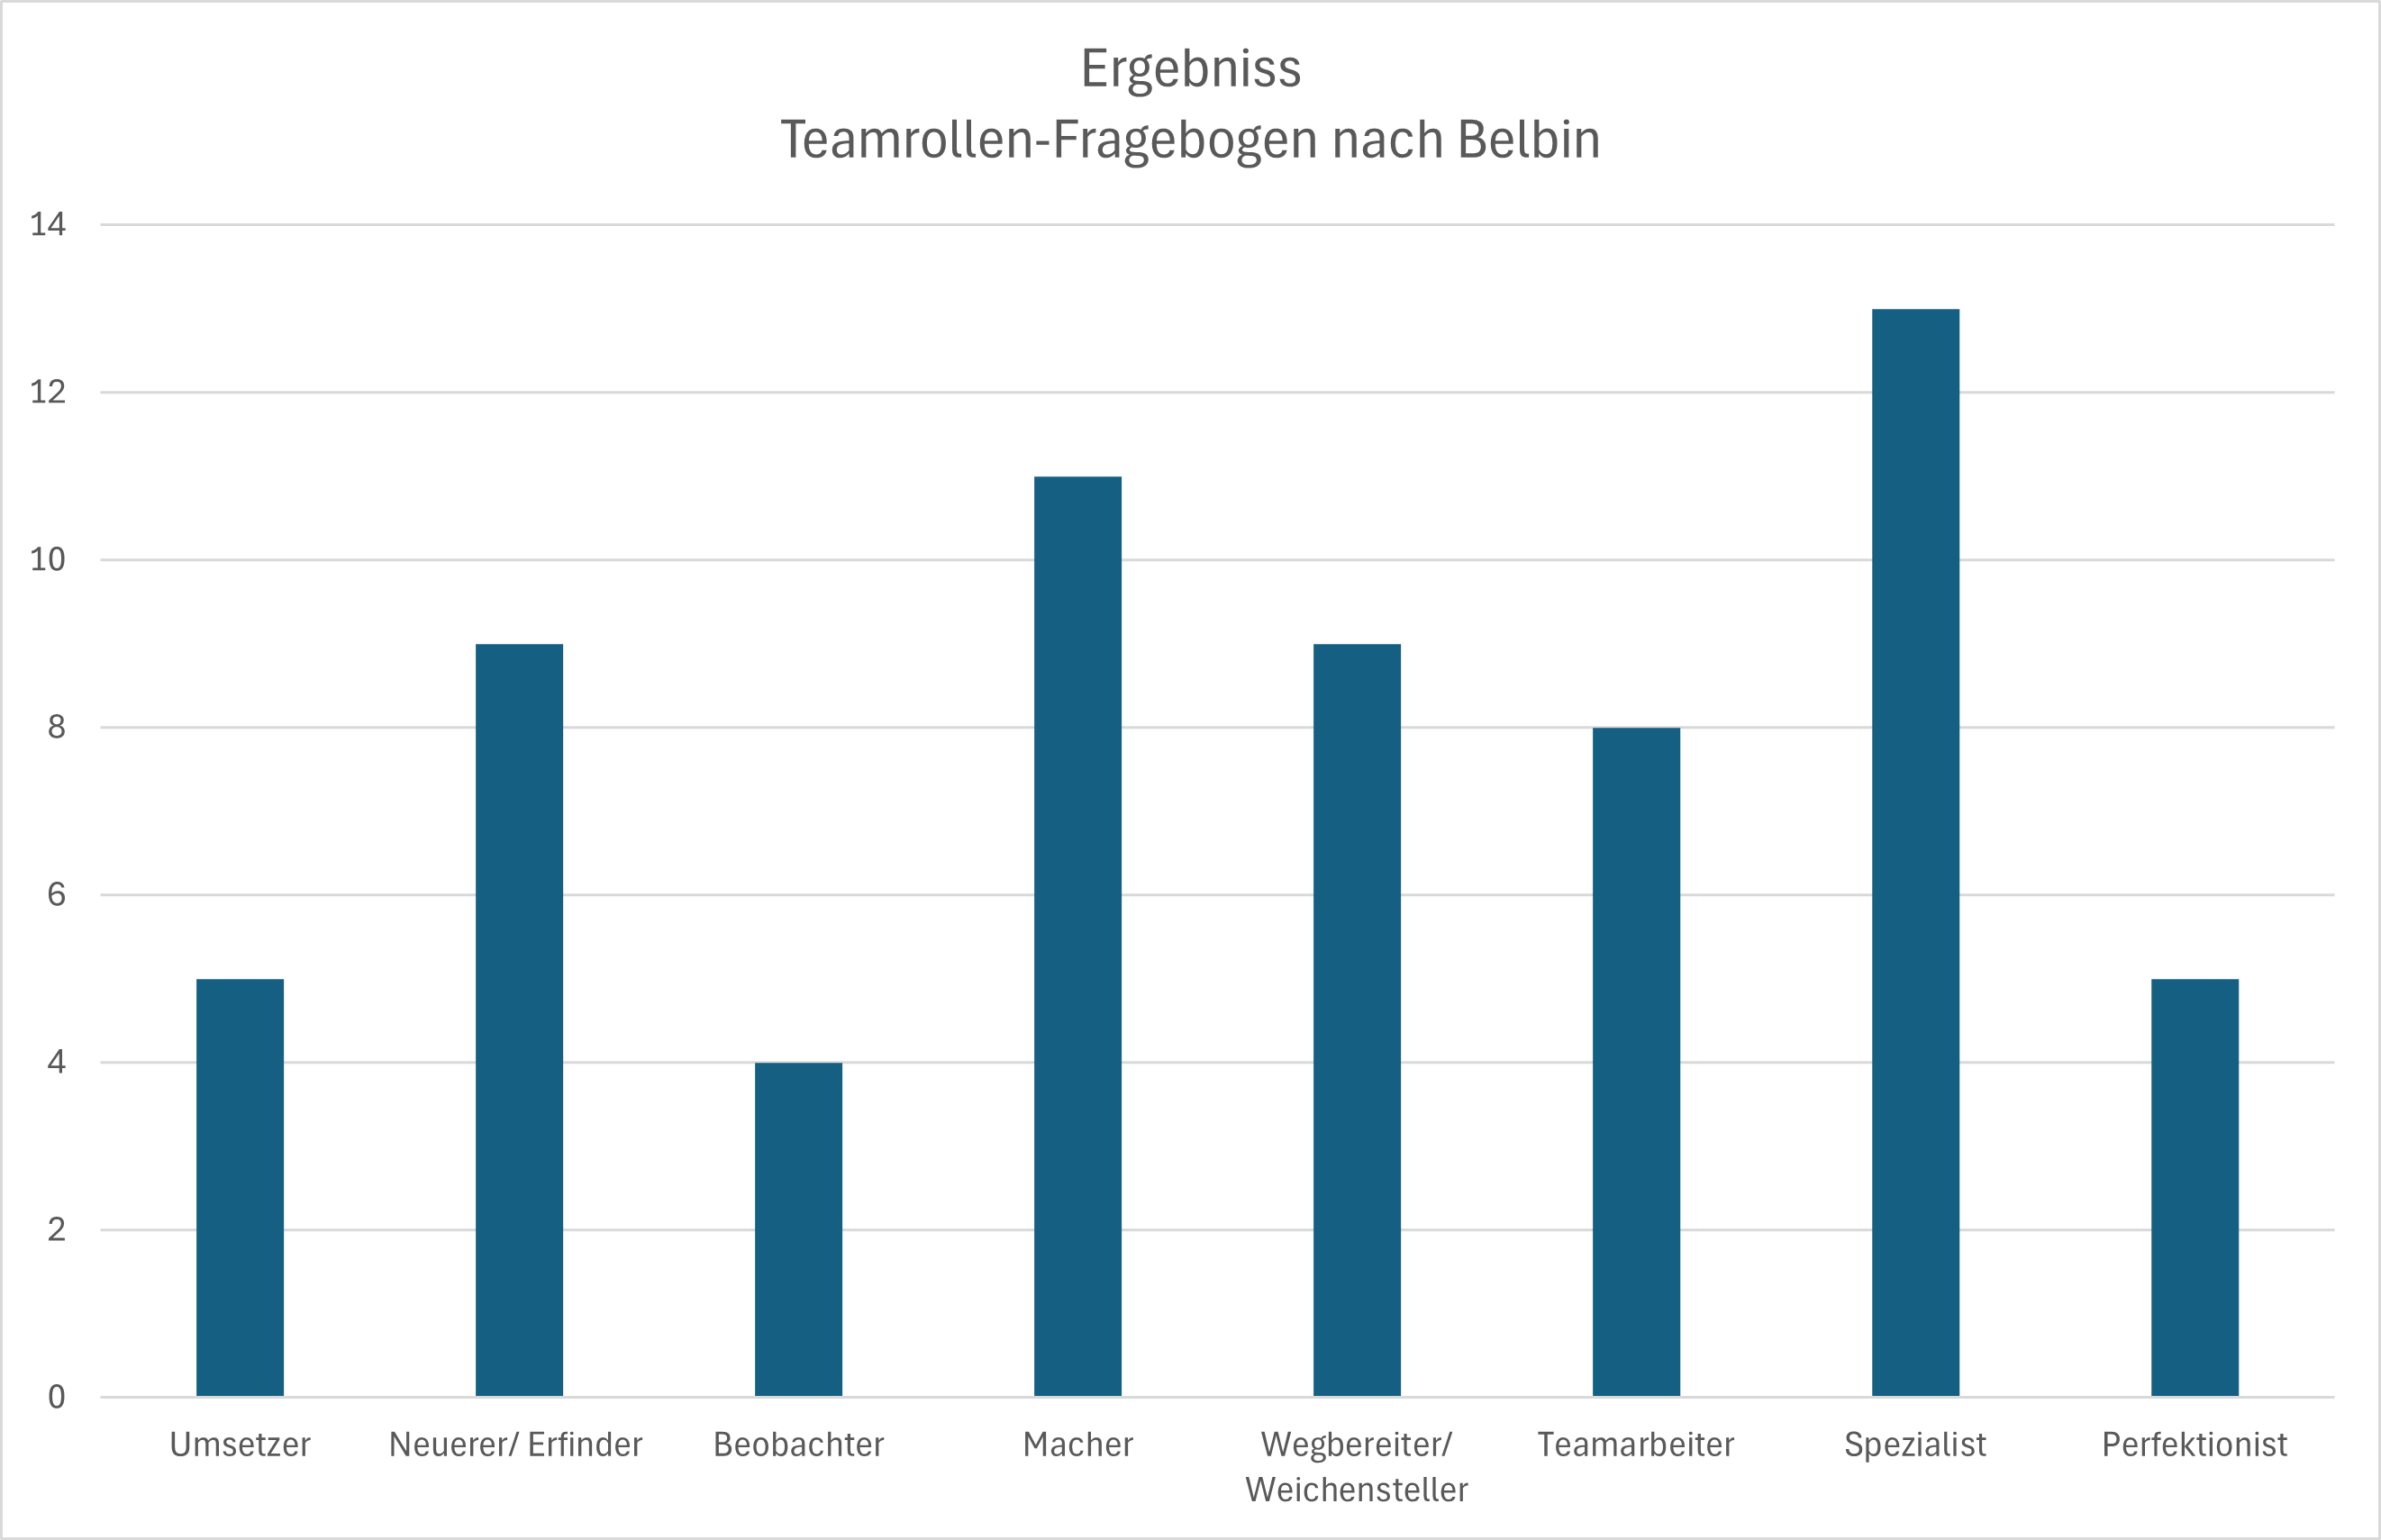
\includegraphics[width=0.8\textwidth]{Pictures/ErgebnisBelbin.png}
    \end{center}
	\caption[Ergebniss Teamrollen-Fragebogen nach Belbin]{Ergebniss Teamrollen-Fragebogen nach Belbin}
	\label{fig:ErgebnisBelbin}
\end{figure}

\newpage

\section{Konfliktlösung}
Um mit der Situation umzugehen, in der ein Projektmitglied wiederholt behauptet, in Meetings schlecht informiert zu werden, würde ich basierend auf den Unterlagen folgende Schritte unternehmen:

\subsection{Konfliktart erkennen}
Es liegt offensichtlich ein Kommunikationskonflikt vor, da das Teammitglied das Gefühl hat, nicht genügend Informationen zu erhalten. In so einem Fall fehlen oft klare Absprachen oder wesentliche Details, die zu Missverständnissen führen.

\subsection{Ursachenanalyse}
Bevor ich das Gespräch suche, würde ich prüfen, ob tatsächlich Informationslücken bestehen oder ob das Problem auf einem Missverständnis beruht. Dazu schaue ich mir an, was bisher kommuniziert wurde, und ob es vielleicht interne Prozesse gibt, die zu Verwirrung geführt haben.

\subsection{Vorbereitung auf das Konfliktgespräch}
Nachdem ich die Lage analysiert habe, würde ich ein zeitnahes Gespräch ansetzen und dem Teammitglied vorab den Grund mitteilen. Dadurch kann es sich auch vorbereiten und es gibt weniger Chancen für Missverständnisse. Eine klare Zielsetzung ist hier wichtig – zum Beispiel zu klären, wie wir die Informationsweitergabe verbessern können.

\subsection{Ablauf des Konfliktgesprächs}
\begin{itemize}
    \item \textbf{Positiver Einstieg}: Das Gespräch würde ich positiv eröffnen, etwa mit \glqq Ich freue mich, dass wir die Gelegenheit haben, die Informationslage im Projekt zu besprechen.\grqq{} So signalisiere ich Offenheit und vermeide eine konfrontative Atmosphäre.
    \item \textbf{Problemanalyse}: Ich würde dem Teammitglied Raum geben, seine Sichtweise ohne Unterbrechung zu schildern, während ich aktiv zuhöre. Das zeigt Verständnis und schafft eine konstruktive Basis.
    \item \textbf{Lösungsfindung}: Im nächsten Schritt suchen wir gemeinsam nach Lösungen. Ich würde mögliche Maßnahmen vorschlagen, z. B. wie Informationen in Zukunft klarer und transparenter bereitgestellt werden können, und die Vereinbarungen schriftlich festhalten.
\end{itemize}

\subsection{Konstruktives Verhalten}
Während des gesamten Gesprächs würde ich \glqq Ich-Botschaften\grqq{} nutzen, um Schuldzuweisungen zu vermeiden. Ein Beispiel: \glqq Mir ist aufgefallen, dass du in den Meetings öfter das Gefühl hast, nicht ausreichend informiert zu sein. Ich möchte besser verstehen, wie wir das optimieren können.\grqq{} Dadurch halte ich das Gespräch sachlich und vermeide Eskalation.


\section{Lego Serious Play}

Die Methode Lego Serious Play (LSP) bietet klare Vorteile, aber auch Nachteile, die je nach Situation berücksichtigt werden müssen.

\subsection{Vorteile der Methode}
\begin{itemize}
    \item \textbf{Visualisierung komplexer Ideen}: LSP ermöglicht es, abstrakte Konzepte durch den Bau von Modellen zu veranschaulichen. Dadurch können Gedanken und Probleme effizienter kommuniziert werden.
    \item \textbf{Förderung von Kreativität und Teamarbeit}: Da jeder Teilnehmer seine Perspektive einbringt, entstehen vielfältige Lösungsansätze, die im Team weiterentwickelt werden.
    \item \textbf{Gleichberechtigung aller Teilnehmer}: Jede Stimme zählt. Die Methode schafft eine Atmosphäre, in der alle Ideen eingebracht und gehört werden, was für eine offene Diskussion sorgt.
\end{itemize}

\subsection{Nachteile der Methode}
\begin{itemize}
    \item \textbf{Zeitaufwand}: Der Prozess erfordert Zeit. Da jeder Teilnehmer seine Modelle erklären muss, kann LSP bei schnelleren Entscheidungsprozessen zu zeitintensiv sein.
    \item \textbf{Begrenzte Tiefe bei komplexen Themen}: Bei sehr technischen oder detaillierten Fragestellungen stößt die Methode an ihre Grenzen.
    \item \textbf{Nicht für jede Gruppe geeignet}: In konservativen oder formellen Umgebungen könnte das spielerische Element auf Ablehnung stoßen und die Effektivität mindern.
\end{itemize}

\subsection{Situative und adaptive Führung}
Durch den Einsatz von LSP habe ich erkannt, wie wichtig es ist, Führung an den Kontext und das Team anzupassen. LSP erfordert ein hohes Maß an Flexibilität, da jede Person ihre eigenen Ideen einbringt. Für mich als Führungskraft bedeutet das, schnell auf verschiedene Kommunikations- und Arbeitsstile reagieren zu können, ohne das gemeinsame Ziel aus den Augen zu verlieren.
Ich habe gelernt, dass adaptive Führung nicht nur darin besteht, Raum für Kreativität zu schaffen, sondern auch die Kontrolle über den Prozess zu behalten. Strukturierte und ergebnisorientierte Führung bleibt der Kern, aber LSP hat mir gezeigt, wann es nötig ist, Kreativität zuzulassen und wann es wichtig ist, wieder klare Vorgaben zu machen.
LSP verdeutlicht, dass situative Führung sowohl das Fördern von Kreativität als auch das Anbieten von Struktur erfordert, um letztlich auf das gemeinsame Ziel hinzuarbeiten.
\newpage
\section{Anwendung der erarbeiteten \glqq einfachen Handlungsrichtlinien\grqq{}}
In der Situation, in der ich ein neues Team übernehme und einer der bestehenden Mitarbeiter öffentlich Unzufriedenheit äußert, würde ich mich auf die zentralen Handlungsrichtlinien konzentrieren, die direkt auf die Herausforderung einzahlen:

\begin{itemize}
    \item \textbf{Offene Tür für die Mitarbeiter haben}: Der erste Schritt wäre ein direktes Gespräch mit dem unzufriedenen Mitarbeiter. Dabei ist es entscheidend, ihm Raum zu geben, seine Bedenken offen zu äußern. Durch aktives Zuhören kann ich seine Perspektive nachvollziehen und gleichzeitig signalisieren, dass ich seine Meinung ernst nehme. Das schafft Vertrauen und verhindert, dass sich der Konflikt weiter zuspitzt.
    \item \textbf{Das Ruder übernehmen und die Mitarbeiter bei sich behalten}: In dieser Phase ist es wichtig, klare Führung zu zeigen. Ich würde dem Team transparent erklären, warum es zu dieser Neuzusammensetzung gekommen ist und welche Ziele damit verfolgt werden. Dadurch stelle ich sicher, dass alle verstehen, dass Veränderungen nicht nur Herausforderungen, sondern auch Chancen mit sich bringen. Meine Rolle ist es, das Team trotz Unstimmigkeiten zusammenzuhalten und den Fokus auf das gemeinsame Ziel zu richten.
    \item \textbf{Brücken zwischen den Mitarbeitern bauen}:Da zwei Mitarbeiter neu im Unternehmen sind und zwei aus anderen Teams kommen, liegt ein klarer Fokus darauf, die Zusammenarbeit zu fördern. Um Konflikten vorzubeugen, würde ich gezielt Maßnahmen ergreifen, um das Team zu integrieren. Dazu könnten Workshops oder kleinere Projekte gehören, bei denen die Mitarbeiter ihre Stärken einbringen und voneinander lernen. Dadurch wird die Zusammenarbeit gefördert und das Team wächst schneller zusammen.
    \item \textbf{Ziele mit den Mitarbeitern zusammen erreichen und sie motivieren}: Um den unzufriedenen Mitarbeiter stärker zu integrieren, würde ich ihm gezielt Verantwortung im Team übertragen. Indem er sieht, dass seine Rolle wichtig ist und sein Beitrag zählt, könnte seine Motivation steigen. Zudem würde ich klar formulieren, welche Ziele wir als Team erreichen wollen, und sicherstellen, dass jeder im Team das Gefühl hat, zu diesem Erfolg beizutragen.
\end{itemize}

Durch diese fokussierte Herangehensweise kann ich sicherstellen, dass der Unmut des Mitarbeiters ernst genommen wird, das Team schnell zusammenwächst und wir gemeinsam an einem Strang ziehen, um unsere Ziele zu erreichen.
\newpage
\section{Konstruktives Feedback}

Die LV-Leiterin hat sich stark bemüht, trotz der Herausforderungen Softskills an Techniker zu vermitteln. Besonders der Einsatz von Lego Serious Play machte den Inhalt praxisnah und verständlicher, was für mich persönlich mehr Mehrwert hatte als klassische PowerPoint-Präsentationen. Dadurch konnte ich deutlich mehr aus der Vorlesung mitnehmen. Dennoch glaube ich, dass diese Skills für viele Teilnehmer nicht wirklich von Relevanz sind. Solche Fähigkeiten werden über die Zeit entwickelt und können nicht in einem einzigen Kurs vollständig vermittelt werden. Bestimmte Menschen haben eine natürliche Eignung für Führungspositionen, während andere weniger dafür geeignet sind.

\newpage

%\input{Chapters/ResultsInterpretation}
%% -> Schlussteil
%\input{Chapters/Conclusions}
%% --------------------------------------------------------------------- %%

\clearpage

%% --------------------------------------------------------------------- %%

%% Aufrufen der Einträge im Symbolverzeichniss
\glsaddall
%% -> Verzeichnisse
\pagestyle{fancy}
\pagenumbering{Roman}
\addtocounter{romanPagenumber}{1}
\setcounter{page}{\theromanPagenumber}

%% --------------------------------------------------------------------- %%

% -> Literaturverzeichnis IEEE-gerecht
\bibliographystyle{IEEEtran}
\renewcommand\refname{Literaturverzeichnis}
\bibliography{Verzeichnisse/Literatur}
\ifthenelse{\boolean{english}}
{\addcontentsline{toc}{section}{Bibliography}}
{\addcontentsline{toc}{section}{Literaturverzeichnis}}
\newpage
%% --------------------------------------------------------------------- %%

%% -> Abbildungsverzeichnis
\listoffigures
\ifthenelse{\boolean{english}}
{\addcontentsline{toc}{section}{List of Figures}}
{\addcontentsline{toc}{section}{Abbildungsverzeichnis}}
\newpage
%% --------------------------------------------------------------------- %%

%% -> Tabellenverzeichnis
%\listoftables 
%\ifthenelse{\boolean{english}}{\addcontentsline{toc}{section}{List of Tables}}
%{\addcontentsline{toc}{section}{Tabellenverzeichnis}}
%\newpage
%% --------------------------------------------------------------------- %%

%% -> Formelverzeichnis
%\listofmyequations
%\ifthenelse{\boolean{english}}{\addcontentsline{toc}{section}{List of Equations}}
%{\addcontentsline{toc}{section}{Formeleverzeichnis}}
%\newpage
%% --------------------------------------------------------------------- %%

%% -> Abkürzungsverzeichnis -> List of Abbreviations <-
%\printglossary[style=My Acronym,type=\acronymtype, title={Abkürzungsverzeichnis}]
%\newpage

%% --------------------------------------------------------------------- %%

%% -> Symbolverzeichnis 
%\printglossary[style=My Symbols,title={Symbolverzeichnis}]

%% --------------------------------------------------------------------- %%


%% --------------------------------------------------------------------- %%
\clearpage
% -> Anhang
 \begin{appendix}
 	\input{Anhang/Anhang}
 \end{appendix}

\end{document}
